%==============================Kapitola: Terminálový vstup a výstup=======================================================  
\chapter{Terminálový vstup a výstup}
\minitoc
\newpage
  Jazyk C, narozdíl od Pascalu, nedefinuje žádnou \texttt{I/O (vstup\-ně/výstup\-ní -In\-put/Out\-put)} operaci jako část jazyka.
  Nezbytné vstupy a výstupy jsou řešeny tak, že standardní knihovna obsahuje několik funkcí, které \texttt{I/O} zajišťují.

  Nejvíce strojově závislé akce jsou I/O operace a tímto způsobem se tedy důsledně oddělují strojově závislé a strojově nezávislé
  části jazyka. Tato skutečnost je pak významným přínosem při vytváření kompilátoru pro jiný počítač.

  \begin{figure}[ht!]
     \centering
     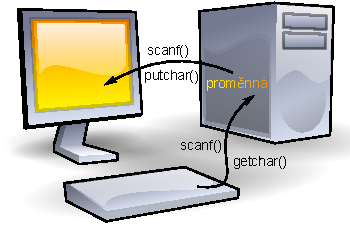
\includegraphics[scale=1.2]{terminalovy_IO_skica.pdf}
     \caption{Operace pro terminálový vstup a výstup}\label{C:fig_Terminal_IO}
  \end{figure}

  \section{Hlavičkový soubor \lstinline[basicstyle=\ttfamily]!stdio.h!}
    Aby bylo možno správně používat všechny funkce pro vstupu a výstupu, je nutné na začátku programu připojit "popis" těchto
    funkcí. Ten se nachází v hlavičkovém (\emph{header}) souboru \lstinline[basicstyle=\ttfamily]!stdio.h!:

    \lstinline[basicstyle=\ttfamily]!#include <stdio.h>  //zde neni strednik!

    Od tohoto okamžiku je pak možné používat dále popsané funkce.

  \section{Standardní vstup a výstup znaku}
    Výstup jednoho znaku zajišťuje \lstinline[basicstyle=\ttfamily]!putchar()! a vstup jednoho znaku funkce
    \lstinline[basicstyle=\ttfamily]!getchar()!.
    \begin{itemize}
      \item \lstinline[basicstyle=\ttfamily]!int putchar(int c);!
      \item \lstinline[basicstyle=\ttfamily]!int getchar(void);!
    \end{itemize}
    Obě funkce pracují s proměnnými \lstinline[basicstyle=\ttfamily]!int! a ne \lstinline[basicstyle=\ttfamily]!char!.

      \marginpar{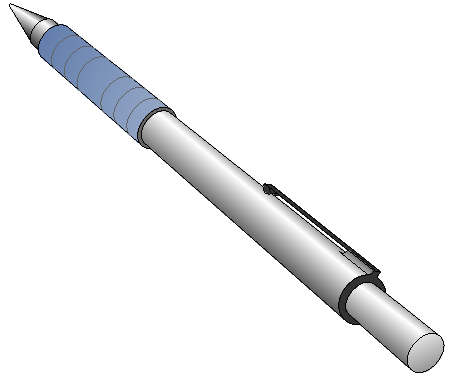
\includegraphics[width=0.09\textwidth]{pen.pdf}}
      %---------------------------------------------------------------
      \lstinputlisting{../src/C/file/Cteni_tisk_znaku.c} 
      \begin{lstlisting}[caption=\texttt{Cteni\_tisk\_znaku.c} Čtení a tisk znak ze standardního vstupu na standardní výstup.]
      \end{lstlisting}
      %--------------------------------------------------------------    
    
    \begin{example}Čtení znaku ze standardního vstupu a jejich zápis na standardní výstup ukazuje následující program,
      představující jednoduchou variantu příkazu kopírování souboru (nutno ovšem přesměrovat vstup a výstup).

      \marginpar{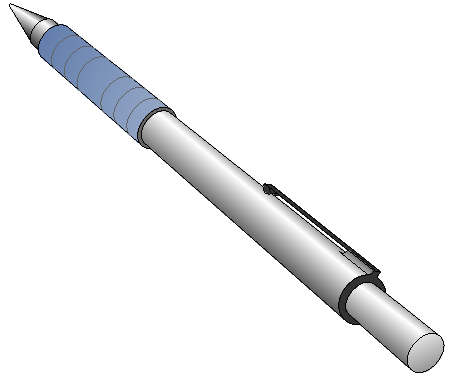
\includegraphics[width=0.09\textwidth]{pen.pdf}}
      %---------------------------------------------------------------
      \lstinputlisting{../src/C/file/CPY.c}
      \begin{lstlisting}[caption=\texttt{CPY.c} Kopíruje znak ze standardního vstupu na standardní výstup.]
      \end{lstlisting}
      %---------------------------------------------------------------
    \end{example}
    
  \section{Standardní vstup a výstup řetězců}
    Standardní vstup a výstup řetězců je jednoduchou nadstavbou nad čtením znaku. Obě funkce,
    \begin{itemize}
      \item \lstinline[basicstyle=\ttfamily]!char *gets(char *s);!
      \item \lstinline[basicstyle=\ttfamily]!int puts(const char *s);!
    \end{itemize}
    pracují s řetězci. \texttt{gets()} načte do znakového pole vstupní řetězec az do konce řádku, symbol
    \lstinline[basicstyle=\ttfamily]!'\n'! není do znakového pole zapsán. Ukazatel na pole (načtený řetězec) je rovněž návratovou
    hodnotou. Chybu signalizuje návrat NULL. \texttt{puts()} zapíše řetězec na výstup a přidá přechod na novy řádek
    \lstinline[basicstyle=\ttfamily]!'\n'!. Chybu představuje návratové \texttt{EOF}, jinak vrací kladné cele číslo.

    Jednoduchost použití skrývá velké nebezpečí. Funkce \texttt{gets()} nemá informaci o délce oblasti vymezené pro čtený
    řetězec. Je-li oblast kratší, než vstupní řádek, dojde jeho načtením velmi pravděpodobně k přepsání paměťové oblasti
    související s vyhrazenou pamětí. A to se všemi důsledky z toho vyplývajícími.


  \section{Formátovaný standardní vstup a vystup}
  \section{Souhrnné cvičení}
    \begin{example}Vytvořte program, který vygeneruje ASCII tabulku se čtyřmi sloupci ve formátu \textbf{[znak|kód|znak|kód]}.
      Rozsah tabulky definujte pomocí dvou symbolických konstant \lstinline[basicstyle=\ttfamily]!MIN_ASCII, MAX_ASCII!.

      \marginpar{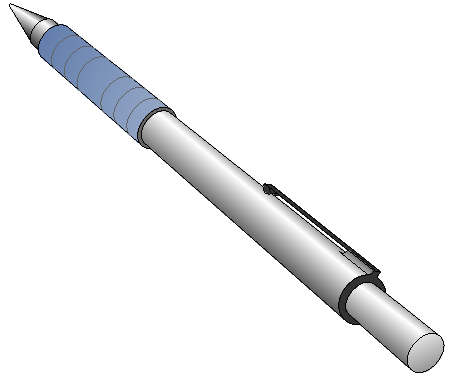
\includegraphics[width=0.09\textwidth]{pen.pdf}}
      %---------------------------------------------------------------
      \lstinputlisting{../src/C/file/ASCII.c}
      \begin{lstlisting}[caption=\texttt{ASCII.c} Generuje ASCII tabulku na terminálu.]
      \end{lstlisting}
      %---------------------------------------------------------------
    \end{example} 